\documentclass[11pt,a4paper]{article}

% Packages
\usepackage[utf8]{inputenc}
\usepackage[T1]{fontenc}
\usepackage{amsmath,amssymb,amsthm}
\usepackage{graphicx}
\usepackage{hyperref}
\usepackage{booktabs}
\usepackage{xcolor}
\usepackage{tikz}
\usetikzlibrary{shapes,arrows,positioning}
\usepackage[margin=1in]{geometry}

% Theorem environments
\newtheorem{definition}{Definition}
\newtheorem{theorem}{Theorem}
\newtheorem{lemma}{Lemma}
\newtheorem{proposition}{Proposition}

% Document info
\title{Augmented Democracy as a Coherence-Constrained Control System\\[0.5em]
\large Governance Infrastructure Under Adversarial Conditions}

\author{Sylvain Cormier\\
Paraxiom Research\\
\texttt{sylvain@paraxiom.org}}

\date{December 2025}

\begin{document}

\maketitle

\begin{abstract}
We present a systems-theoretic framework for democratic governance that treats
legitimacy as the preservation of coherence in decision-making processes rather
than as a direct consequence of majority outcomes. The framework introduces
\emph{procedural infrastructure}---including token-curated test grids, dynamic
credential NFTs, and bounded voting weights---that restrict participation to
actors who can demonstrate verifiable engagement with relevant evidence,
\textbf{without assigning semantic authority to the system itself}.

Building on prior work in Hamiltonian machine learning (ERLHS), geometric
consensus (Karmonic Mesh), and quantum-safe validation (Proof of Coherence),
we formalize augmented democracy as a control system in which proposals are
state transitions, participants act as distributed sensors with bounded influence,
and acceptance requires satisfaction of both a democratic majority condition and
a coherence threshold measuring process consistency.

The central claim is that \textbf{democratic legitimacy is a measurable property
of process quality---independent of specific outcomes}---and that governance
systems designed around procedural admissibility and coherence constraints exhibit
improved resistance to manipulation, Sybil attacks, plutocratic capture, and
coordinated adversarial behavior.
\end{abstract}

\tableofcontents
\newpage

%==============================================================================
\section{Problem: Democracy Under Adversarial Load}
\label{sec:problem}
%==============================================================================

Democratic systems face compounding failure modes in the information age. These
failures are not political in nature---they are \textit{systems failures} that
require engineering solutions.

\subsection{The Five Failure Modes}

\paragraph{Unengaged Voting.}
Participants vote without verifiable engagement with proposal-relevant evidence.
In traditional systems, nothing prevents a voter from casting a ballot on a
complex policy question without having read a single document about it. The
resulting signal is noise, not preference revelation.

\paragraph{Coordinated Manipulation.}
Influence campaigns exploit cognitive biases at scale. Social media amplification,
bot networks, and targeted advertising can shift public opinion without any
engagement with factual evidence. The democratic process becomes a contest of
manipulation rather than deliberation.

\paragraph{Speed vs.\ Legitimacy Tradeoff.}
Digital communication enables rapid decision-making, but legitimate deliberation
requires time. Systems optimized for speed sacrifice the careful consideration
that gives decisions their legitimacy. The result is ``fast wrong'' instead of
``slow right.''

\paragraph{AI-Generated Influence.}
Large language models enable scalable persuasion. A single adversary can generate
thousands of personalized, convincing arguments. The asymmetry between offense
(generating influence) and defense (verifying authenticity) favors attackers.

\paragraph{Quantum-Era Threats.}
Future adversaries with quantum computers can retroactively compromise classical
cryptographic commitments. Decisions made today with ECDSA signatures may be
forgeable in a decade. Governance infrastructure must be quantum-resistant from
the start.

\subsection{Why Traditional Responses Fail}

Traditional responses to these failures---education, regulation, fact-checking---address
symptoms rather than architecture.

\begin{itemize}
    \item \textbf{Education} assumes voters will become informed given sufficient
    resources. But rational ignorance~\cite{downs1957economic} suggests voters
    have no individual incentive to invest in becoming informed.

    \item \textbf{Regulation} assumes platforms can be forced to reduce manipulation.
    But platform incentives align with engagement, not accuracy, and regulatory
    capture is endemic.

    \item \textbf{Fact-checking} assumes authoritative sources can determine truth.
    But ``who fact-checks the fact-checkers?'' leads to infinite regress, and
    institutional trust has collapsed across the political spectrum.
\end{itemize}

We require a different approach: treating democracy as \textit{critical infrastructure}
subject to engineering constraints, with formal guarantees that do not depend on
participant virtue or institutional trustworthiness.

%==============================================================================
\section{Philosophical Foundations: Artifacts, Not Truth}
\label{sec:philosophy}
%==============================================================================

Before presenting the technical framework, we establish a critical philosophical
distinction that underlies the entire system.

\subsection{The Semantic Authority Problem}

Any system that claims to determine ``what is true'' faces an infinite regress:
who verifies the verifiers? Classical epistemic gatekeeping (expert panels,
editorial boards, fact-checkers) ultimately rests on institutional authority
that can be captured, corrupted, or contested.

Consider the problem concretely:
\begin{itemize}
    \item If we say ``experts determine facts,'' we must answer: which experts?
    Selected by whom? Accountable to whom?
    \item If we say ``consensus determines facts,'' we must answer: consensus of
    whom? Over what time period? Weighted how?
    \item If we say ``evidence determines facts,'' we must answer: evidence judged
    by whom? According to what standards?
\end{itemize}

Every answer leads to another question. There is no non-circular foundation for
semantic authority.

\subsection{The Solution: Procedural Authority}

Our framework sidesteps this problem entirely. The system makes no semantic
judgments. It enforces \textit{procedural constraints} on what evidence may be
referenced and measures \textit{statistical properties} of the decision process.

This is not a weakness but a design requirement. A system that claimed semantic
authority would be both philosophically indefensible and practically capturable.

\subsection{Admissible Artifacts}

\begin{definition}[Admissible Fact Artifact]
In this framework, a \emph{fact} is not treated as a semantic claim or assertion,
but as a verifiable artifact with cryptographic provenance.
An artifact is admissible for use in governance processes if it satisfies:
\begin{enumerate}
    \item \textbf{Immutable referenceability}: the artifact can be uniquely
    identified via a hash, DOI, or equivalent content-addressed reference;
    \item \textbf{Authentic issuance}: the artifact is bound to a recognized
    issuer, authority, or origin via digital signatures or equivalent mechanisms;
    \item \textbf{Contextual relevance}: the artifact belongs to an artifact
    class declared relevant for the proposal type under consideration.
\end{enumerate}
No semantic interpretation, truth evaluation, or correctness judgment is
performed by the governance system itself.
\end{definition}

This definition has important consequences:

\begin{itemize}
    \item A peer-reviewed paper is admissible because it has a DOI, is signed by
    a journal, and belongs to the ``scientific literature'' artifact class---not
    because its conclusions are ``true.''

    \item A government report is admissible because it has a document ID, is
    signed by an agency, and belongs to the ``official statistics'' artifact
    class---not because its numbers are ``correct.''

    \item A dissenting scientific paper is equally admissible to a consensus paper,
    provided both have valid provenance. The system does not adjudicate which is
    ``right.''

    \item Participants demonstrate engagement with admissible artifacts, not
    agreement with their conclusions.
\end{itemize}

\subsection{Test Grids as Admissibility Registries}

\begin{definition}[Token-Curated Test Grid]
A Token-Curated Test Grid (TCTG) is a governed registry that specifies which
classes of admissible artifacts may be referenced for a given proposal
domain.
Curation decisions are made by participants who stake tokens and are subject to
economic penalties if admitted artifacts are later shown to be malformed,
inauthentic, or procedurally invalid.

Test grids govern \emph{admissibility criteria} (format, provenance, relevance),
not semantic conclusions or interpretations.
\end{definition}

\textbf{Critical distinction}: Test grids do not define truth; they define the set
of artifacts that a decision process is permitted to reference.

Curators are slashed for admitting artifacts that:
\begin{itemize}
    \item Have invalid provenance (forged signatures, broken hash references)
    \item Violate format requirements (wrong artifact class for proposal type)
    \item Were retracted or invalidated by their issuing authority
\end{itemize}

Curators are \textit{not} slashed for admitting artifacts whose conclusions are
later contested, revised, or overturned through normal scientific or institutional
processes. The system does not adjudicate semantic disputes.

\subsection{Coherence as Process Quality}

\begin{definition}[Process Coherence]
The coherence score $\gamma$ does not measure correctness, factual truth, or
proposal merit. It measures statistical consistency and entropy quality of the
decision process given the declared admissible evidence and participation constraints.

Low coherence indicates process instability, coordinated behavior, or insufficient
entropy, independent of proposal content.
\end{definition}

A proposal can have high coherence and still be ``wrong'' by external standards.
A proposal can have low coherence despite being ``correct.'' The coherence score
measures whether the \textit{process} that produced the decision exhibited
properties consistent with legitimate deliberation.

\subsection{Scope of System Authority}

The governance system constrains \emph{how} decisions are made, not \emph{what}
decisions must conclude.

\begin{center}
\begin{tabular}{ll}
\toprule
\textbf{System Does} & \textbf{System Does Not} \\
\midrule
Verify artifact provenance & Evaluate artifact truth \\
Enforce participation requirements & Determine correct outcomes \\
Measure process consistency & Judge proposal merit \\
Bound individual influence & Override collective judgment \\
Detect coordinated manipulation & Censor unpopular positions \\
\bottomrule
\end{tabular}
\end{center}

This scope limitation is not a weakness but a design requirement. A system that
claimed semantic authority would be both philosophically indefensible and
practically capturable.

%==============================================================================
\section{Augmented Democracy: Definition}
\label{sec:definition}
%==============================================================================

\subsection{What Augmented Democracy Is Not}

Before defining what augmented democracy \textit{is}, we clarify what it is
\textit{not}:

\begin{itemize}
    \item \textbf{Not technocracy}: Experts do not override participants. The system
    ensures engagement with evidence, not deference to expert opinion.

    \item \textbf{Not algorithmic rule}: No AI makes final decisions. The algorithm
    enforces process constraints; humans make substantive choices.

    \item \textbf{Not censorship}: All proposals enter the system. The filtering
    occurs on \textit{participation}, not \textit{content}.

    \item \textbf{Not plutocracy}: Wealth does not determine influence. Quadratic
    costs and reputation caps bound the advantage of resources.

    \item \textbf{Not truth arbitration}: The system does not determine what is
    ``true.'' It determines what is procedurally valid.
\end{itemize}

\subsection{Formal Definition}

\begin{definition}[Augmented Democracy]
A \textbf{constrained participation system} with admissibility gates, where:
\begin{enumerate}
    \item Participation requires registration (identity binding via dynamic NFTs)
    \item Voters must demonstrate engagement with proposal-relevant admissible artifacts
    \item Proposals traverse a filtering pipeline (review period with gatherers/curators)
    \item Votes are weighted by reputation and bounded by quadratic costs
    \item Acceptance requires coherence threshold satisfaction (process quality)
    \item All transitions produce cryptographic proofs (auditability)
    \item Credentials decay without ongoing participation (life-sustaining NFTs)
\end{enumerate}
\end{definition}

The key distinction from classical democracy: legitimacy derives from \textit{process invariants},
not outcome ratification. The ``augmented'' refers to procedural augmentation---ensuring voters
have verifiably engaged with relevant evidence before their input shapes collective decisions.

\subsection{The Augmentation Hierarchy}

Different engagement levels are supported:

\begin{center}
\begin{tabular}{lll}
\toprule
\textbf{Role} & \textbf{Engagement} & \textbf{Responsibility} \\
\midrule
Voter & Pass engagement verification & Reputation stake \\
Contributor & Add sources to proposals & Token compensation \\
Gatherer & Identify admissible artifacts & Quality incentives \\
Curator & Assemble test grids & Token stake (slashable) \\
Validator & Verify coherence & Block rewards \\
\bottomrule
\end{tabular}
\end{center}

Users self-select into roles based on desired involvement level.

%==============================================================================
\section{The Coherence Pipeline}
\label{sec:pipeline}
%==============================================================================

The augmented democracy system operates as a six-stage pipeline where each
stage gates the next. This is not a collection of mechanisms but a
\textit{processing pipeline} with formal invariants at each transition.

\begin{figure}[ht]
\centering
\includegraphics[width=0.95\textwidth]{diagrams/coherence-pipeline.pdf}
\caption{The Coherence Pipeline: Six stages with five gates. Each gate must pass
for the proposal to advance. Failure at any gate halts progression without
corrupting state.}
\label{fig:pipeline}
\end{figure}

\subsection{Stage 1: Proposal Creation}

A registered \texttt{Submitter} creates a proposal. The submitter must hold a
valid credential NFT with the \texttt{Submitter} role. Proposals enter the
system in \texttt{Submitted} status.

\textbf{Gate}: Valid submitter credential\\
\textbf{On failure}: Proposal rejected immediately

\subsection{Stage 2: Review Period}

Proposals enter a mandatory review period. During review:
\begin{itemize}
    \item Reviewers assess proposal clarity and scope
    \item Duplicate or malformed proposals are flagged
    \item Community can signal concerns
\end{itemize}

Proposals that survive the review period advance to \texttt{ReadyForVoting}.

\textbf{Gate}: Review period completes without rejection\\
\textbf{On failure}: Proposal held for revision

\textbf{Coherence dimension}: Temporal coherence---deliberation has minimum dwell time.

\subsection{Stage 3: Grid Curation}

Parallel to review, credentialed \textbf{Gatherers} and \textbf{Curators} build the test grid:

\begin{enumerate}
    \item Gatherers identify admissible artifacts: documents with valid provenance
    from recognized issuers (journals, agencies, standards bodies)
    \item Curators assemble artifacts into engagement verification grids
    \item Curators stake tokens on grid quality
    \item Grid is published and linked to the proposal
\end{enumerate}

\textbf{Gate}: Curator stake sufficient, grid properly formed\\
\textbf{On failure}: Grid flagged, new curators assigned

\textbf{Coherence dimension}: Procedural coherence---the artifact registry is curated
by accountable participants with skin in the game.

\subsection{Stage 4: Engagement Verification}

Before voting, each participant must demonstrate engagement with proposal-relevant artifacts.

The engagement verification:
\begin{itemize}
    \item Does not measure intelligence or political alignment
    \item Verifies that the voter has \textit{encountered} the admissible artifacts
    \item Allows disagreement with artifact conclusions
\end{itemize}

\textbf{Critical clarification}: A voter who has engaged with the evidence and
\textit{disagrees} with its conclusions still passes the gate. The system verifies
engagement, not agreement.

\textbf{Gate}: Engagement threshold met\\
\textbf{On failure}: Voter ineligible for this proposal; may retry after review

\subsection{Stage 5: Weighted Voting}

Eligible voters cast weighted votes. Vote weight is a function of:
\begin{enumerate}
    \item \textbf{Reputation}: Accumulated from contributions, engagement verifications, prior participation
    \item \textbf{Quadratic cost}: Multiple votes on same proposal cost $n^2$
    \item \textbf{Quantum entropy}: $\pm 10\%$ randomization prevents prediction
\end{enumerate}

\textbf{Gate}: Signature valid, not a duplicate\\
\textbf{On failure}: Vote rejected

\subsection{Stage 6: Coherence Check and Result}

After the voting period, finalization computes the result. Two conditions must
\textbf{both} be satisfied:

\begin{enumerate}
    \item \textbf{Democratic condition}: $w_{\text{approve}} > w_{\text{reject}}$
    \item \textbf{Coherence condition}: $\gamma > 50$
\end{enumerate}

\textbf{Gate}: Both conditions satisfied\\
\textbf{On failure}: No state change; may investigate and revote

\subsection{Why Both Gates Are Necessary}

\begin{center}
\begin{tabular}{lcc}
\toprule
\textbf{Attack} & \textbf{Blocked by Engagement} & \textbf{Blocked by $\gamma$} \\
\midrule
Unengaged voting & \checkmark & --- \\
Sybil (fake identities) & Partial & \checkmark \\
Coordinated manipulation & --- & \checkmark \\
Bribery & --- & \checkmark \\
Credential theft & --- & \checkmark \\
Bot voting & \checkmark & \checkmark \\
\bottomrule
\end{tabular}
\end{center}

\begin{itemize}
    \item \textbf{Admissibility gate}: Ensures voters have \textit{encountered} relevant artifacts
    \item \textbf{Coherence gate} ($\gamma$): Ensures votes are \textit{statistically independent}
\end{itemize}

A voter who demonstrates engagement but coordinates with others will trigger low $\gamma$.
A voter who votes independently but hasn't engaged fails the admissibility gate.
Both gates must pass for legitimate outcomes.

%==============================================================================
\section{Procedural Infrastructure}
\label{sec:infrastructure}
%==============================================================================

This section describes the infrastructure components that implement the coherence
pipeline.

\subsection{Token-Curated Test Grids}

Following the KILT Protocol model~\cite{kilt2020}, test grids employ three distinct roles:

\begin{enumerate}
    \item \textbf{Claimer}: A participant who asserts readiness to vote on a proposal
    \item \textbf{Attester}: A curator who has assembled the test grid for that proposal
    \item \textbf{Verifier}: The system that checks engagement verification completion
\end{enumerate}

This separation prevents conflicts of interest: those who create tests do not
administer them, and those who verify do not profit from outcomes.

\subsubsection{Gatherers and Curators}

Within the Attester role, two sub-functions operate:

\begin{itemize}
    \item \textbf{Gatherers}: Identify admissible artifacts for a proposal---documents
    with valid provenance from recognized issuers. Gatherers are compensated per
    artifact that meets admissibility criteria.

    \item \textbf{Curators}: Assemble gathered artifacts into engagement verification
    grids. The goal is to confirm that voters have \textit{encountered} the relevant
    evidence, not that they agree with it. Curators stake tokens on grid quality.
\end{itemize}

\subsubsection{Economic Incentives and Slashing}

\textbf{Slashing conditions} (curators lose staked tokens):
\begin{itemize}
    \item Admitting artifacts with invalid provenance (forged signatures, broken hashes)
    \item Admitting artifacts from non-recognized issuers
    \item Admitting artifacts outside the declared artifact class
    \item Admitting artifacts that were retracted by their issuing authority
\end{itemize}

\textbf{Not slashable} (curators are protected):
\begin{itemize}
    \item Admitting artifacts whose conclusions are later contested or revised
    \item Admitting artifacts that some participants disagree with
    \item Admitting artifacts from one scientific position when others exist
\end{itemize}

The system does not adjudicate semantic disputes. Curators are accountable for
\textit{procedural validity}, not \textit{correctness}.

\subsection{Dynamic Credential NFTs}

Participant credentials are not static. A voter's eligibility, weight, and
privileges evolve based on contribution history through \textbf{Dynamic NFTs}---non-fungible
tokens whose metadata updates based on on-chain activity.

The credential NFT updates automatically when:
\begin{itemize}
    \item An engagement verification is passed or failed
    \item A vote is cast
    \item A proposal is submitted
    \item Reputation is adjusted by peer review
    \item Domain certification is earned or revoked
\end{itemize}

\subsubsection{Life-Sustaining NFTs}

A critical innovation is the \textbf{Life-Sustaining NFT}---a credential that requires
ongoing activity to remain valid. Unlike static credentials that persist indefinitely,
life-sustaining NFTs decay without continuous participation.

This addresses the ``ghost voter'' problem: credentials issued to participants who
subsequently disengage. By requiring periodic activity (voting, contributing,
engagement verification), the system ensures that voting weight reflects
\textit{active} participation, not historical registration.

\subsubsection{Domain-Specific Credentials}

Voters may hold credentials in specific domains:

\begin{center}
\begin{tabular}{ll}
\toprule
\textbf{Domain} & \textbf{Unlocks Voting On} \\
\midrule
Environmental & Climate, conservation, pollution proposals \\
Technical & Infrastructure, protocol upgrades \\
Economic & Treasury, tokenomics, funding proposals \\
Social & Community guidelines, dispute resolution \\
Emergency & Crisis response, security incidents \\
\bottomrule
\end{tabular}
\end{center}

Domain credentials are earned by passing domain-specific engagement verifications
and maintained through ongoing participation.

\subsection{Quadratic Voting for Bounded Influence}

The framework incorporates \textbf{quadratic voting} to prevent plutocratic capture
while preserving signal strength for high-conviction preferences.

\subsubsection{The Quadratic Cost Function}

The cost to cast $n$ votes on a single proposal from a single participant:
\begin{equation}
    \text{cost}(n) = n^2
\end{equation}

\begin{center}
\begin{tabular}{ccc}
\toprule
\textbf{Votes Cast} & \textbf{Cost} & \textbf{Marginal Cost} \\
\midrule
1 & 1 & 1 \\
2 & 4 & 3 \\
3 & 9 & 5 \\
4 & 16 & 7 \\
5 & 25 & 9 \\
\bottomrule
\end{tabular}
\end{center}

The increasing marginal cost discourages concentration of voting power on single
proposals, encouraging participants to distribute influence across multiple issues.

\subsubsection{Whale Resistance}

Consider an adversary with 100$\times$ the resources of an average participant:

\begin{center}
\begin{tabular}{lcc}
\toprule
\textbf{System} & \textbf{Adversary Influence} & \textbf{Ratio} \\
\midrule
1-person-1-vote & 1 vote & 1:1 \\
Plutocratic (1:1 stake) & 100 votes & 100:1 \\
Quadratic & 10 votes & 10:1 \\
Quadratic + Reputation Cap & $\leq$ 10 votes & $\leq$ 10:1 \\
\bottomrule
\end{tabular}
\end{center}

Quadratic voting reduces the 100:1 wealth advantage to a 10:1 voting advantage.
Combined with reputation caps and coherence thresholds, adversarial influence
is further bounded.

%==============================================================================
\section{Governance as a Control System}
\label{sec:control}
%==============================================================================

Democratic governance can be formally modeled as a control system with specific
invariants that must be preserved across state transitions.

\subsection{The Control-Theoretic View}

\begin{definition}[Governance Control System]
A tuple $(S, A, T, I, R)$ where:
\begin{itemize}
    \item $S$: State space (current policy/system configuration)
    \item $A$: Action space (proposals as potential state transitions)
    \item $T: S \times A \rightarrow S$: Transition function (proposal execution)
    \item $I$: Coherence invariant (must hold for valid transitions)
    \item $R$: Rejection mechanism (blocks invalid transitions)
\end{itemize}
\end{definition}

\begin{figure}[ht]
\centering
\includegraphics[width=0.9\textwidth]{diagrams/control-loop.pdf}
\caption{Governance as a Control Loop. Participants act as distributed sensors;
credentials provide gain functions; the coherence check ($\gamma > 50$) gates
state transitions.}
\label{fig:control}
\end{figure}

\subsection{Participants as Sensors}

In control theory, sensors measure system state. In governance, participants
provide distributed measurement of collective preference. Unlike physical sensors,
governance sensors are:

\begin{itemize}
    \item \textbf{Heterogeneous}: Each participant has different information access
    \item \textbf{Strategic}: Participants may misreport to influence outcomes
    \item \textbf{Bounded}: Each participant sees only part of the system
\end{itemize}

The framework addresses these properties through credential-weighted aggregation
and coherence-based filtering.

\subsection{The Dual Condition}

The central contribution is the dual-condition consensus requirement. Approval
requires \textbf{both}:

\begin{enumerate}
    \item $w_{\text{approve}} > w_{\text{reject}}$ (democratic condition)
    \item $\gamma > 50$ (coherence condition)
\end{enumerate}

where $\gamma$ is the \textit{quantum confidence score}, computed as:

\begin{equation}
    \gamma = \min\left(\frac{\sigma^2_\eta}{255}, 1\right) \times 100
\end{equation}

and $\sigma^2_\eta$ is the variance of entropy values across votes.

\textbf{Key insight}: Low variance indicates correlated votes (Sybil attack,
coordination, bribery). High variance indicates independent voting (legitimate process).

\subsection{Coherence as Lyapunov Function}

The coherence threshold acts as a Lyapunov function. States with $\gamma \leq 50$
are \textit{outside the coherence manifold}---they may satisfy the democratic
condition but fail the process quality invariant.

The system refuses to transition to such states, even under majority pressure.
This inverts the traditional democratic assumption: legitimacy is not derived
from majority agreement alone, but from the quality of the process that produced
the agreement.

\subsection{Bounded Influence}

No single participant can dominate outcomes. The weight function satisfies:
\begin{equation}
    w_i \in [w_{\min}, w_{\max}] \quad \forall i
\end{equation}

with $w_{\min} = 1$ (floor) and $w_{\max} = r_i \cdot 1.1$ (reputation cap with
10\% entropy bonus maximum).

\subsection{Rollback and Retry Semantics}

Failed coherence checks do not corrupt state. The system remains at $s_t$ when:
\begin{itemize}
    \item $w_{\text{approve}} \leq w_{\text{reject}}$ (democratic failure)
    \item $\gamma \leq 50$ (coherence failure)
    \item Entropy pool exhausted (resource failure)
\end{itemize}

Submitters may revise and resubmit. The state machine supports retry without penalty.

%==============================================================================
% Coherence as Layered Invariant - connects procedural, geometric, and quantum coherence
%==============================================================================
%==============================================================================
% SECTION: Coherence as Layered Invariant
% Insert after Section 6 (Governance as Control System) or before Threat Model
%==============================================================================

\section{Coherence as Layered Invariant}
\label{sec:coherence-layers}

The term \emph{coherence} appears across multiple domains in distributed systems, from quantum physics to machine learning to governance. This section clarifies how procedural coherence ($\gamma$) relates to these other usages and argues that coherence preservation is a unifying principle across the full system stack.

\subsection{Three Layers of Coherence}

We identify three distinct but related coherence concepts:

\begin{definition}[Quantum Coherence]
In quantum information systems, coherence refers to the preservation of phase relationships between quantum states. A quantum channel maintains coherence when superposition states survive transmission without collapsing into classical mixtures. Formally, for density matrix $\rho$:
\[
\mathcal{C}_q(\rho) = \sum_{i \neq j} |\rho_{ij}|
\]
measures the off-diagonal elements that encode quantum correlations. Decoherence---the loss of these correlations through environmental interaction---degrades channel capacity and security guarantees in protocols like QKD.
\end{definition}

\begin{definition}[Geometric Coherence]
In representation learning and neural architectures, coherence refers to the preservation of semantic relationships in embedding spaces. A model maintains geometric coherence when:
\begin{enumerate}
    \item Similar inputs map to proximate regions of the embedding manifold
    \item Semantic operations (analogy, composition) correspond to geometric operations
    \item The manifold structure remains stable under perturbation
\end{enumerate}
Geometric incoherence manifests as embedding drift, manifold collapse, or semantic inconsistency---conditions where the model's internal representations no longer faithfully encode the relationships they purport to represent.
\end{definition}

\begin{definition}[Procedural Coherence]
In governance systems, coherence refers to the statistical properties of decision processes that indicate authentic, independent participation. As defined in Section~\ref{sec:pipeline}, the procedural coherence score:
\[
\gamma = \frac{\sigma^2_\eta}{255} \times 100
\]
measures entropy-weighted variance in voting patterns. Low $\gamma$ indicates coordinated behavior inconsistent with independent decision-making.
\end{definition}

\subsection{The Coherence Stack}

These three coherence types form a dependency hierarchy in systems that span physical infrastructure through algorithmic mediation to collective decision-making:

\begin{figure}[h]
\centering
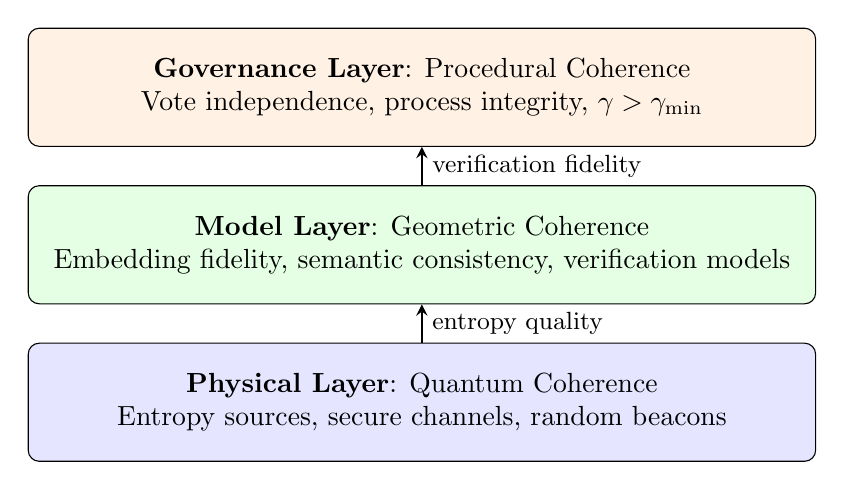
\begin{tikzpicture}[
    layer/.style={rectangle, draw, rounded corners, minimum width=10cm, minimum height=1.5cm, align=center},
    arrow/.style={->, thick, >=stealth}
]
\node[layer, fill=blue!10] (phys) at (0,0) {\textbf{Physical Layer}: Quantum Coherence\\Entropy sources, secure channels, random beacons};
\node[layer, fill=green!10] (model) at (0,2) {\textbf{Model Layer}: Geometric Coherence\\Embedding fidelity, semantic consistency, verification models};
\node[layer, fill=orange!10] (gov) at (0,4) {\textbf{Governance Layer}: Procedural Coherence\\Vote independence, process integrity, $\gamma > \gamma_{\min}$};

\draw[arrow] (phys) -- node[right, font=\small] {entropy quality} (model);
\draw[arrow] (model) -- node[right, font=\small] {verification fidelity} (gov);
\end{tikzpicture}
\caption{The coherence stack: each layer depends on coherence preservation in layers below.}
\label{fig:coherence-stack}
\end{figure}

\textbf{Physical $\to$ Model}: The entropy injection mechanism ($\epsilon \sim \pm 10\%$) that enables procedural coherence detection relies on high-quality randomness. If quantum entropy sources suffer decoherence, the resulting pseudo-randomness may exhibit patterns that either (a) fail to distinguish authentic from coordinated voting, or (b) introduce false positives by injecting correlated noise. Quantum coherence in the entropy generation layer is thus a precondition for meaningful $\gamma$ measurement.

\textbf{Model $\to$ Governance}: If test grid verification or artifact validation employs machine learning models (e.g., for semantic relevance checking, engagement verification, or anomaly detection), geometric coherence in those models affects governance outcomes. A model with collapsed embeddings may fail to distinguish substantively different proposals; a model with drifted representations may inconsistently apply admissibility criteria. Geometric coherence in the model layer is thus a precondition for consistent procedural application.

\subsection{Coherence Degradation Propagates Upward}

A critical property of the coherence stack is that degradation propagates upward but not downward:

\begin{proposition}[Upward Propagation]
Let $\mathcal{C}_q$, $\mathcal{C}_g$, and $\gamma$ denote quantum, geometric, and procedural coherence respectively. Then:
\[
\mathcal{C}_q < \mathcal{C}_q^{\min} \implies \mathbb{E}[\gamma] < \gamma_{\text{authentic}}
\]
and
\[
\mathcal{C}_g < \mathcal{C}_g^{\min} \implies \text{Var}[\gamma] > \text{Var}_{\text{expected}}
\]
That is, quantum decoherence biases procedural coherence measurements, and geometric incoherence increases their variance.
\end{proposition}

This has practical implications: a governance system cannot achieve reliable procedural coherence guarantees without monitoring coherence at lower layers. The $\gamma > 50$ threshold assumes baseline coherence in entropy sources and verification models.

\subsection{Unified Interpretation}

Despite domain-specific formalizations, all three coherence types share a common interpretation:

\begin{quote}
\emph{Coherence measures the degree to which a system preserves the structure it claims to preserve.}
\end{quote}

\begin{itemize}
    \item \textbf{Quantum}: Preserves superposition structure through transmission
    \item \textbf{Geometric}: Preserves semantic structure through embedding
    \item \textbf{Procedural}: Preserves independence structure through aggregation
\end{itemize}

In each case, coherence loss indicates that the system's outputs no longer faithfully represent its inputs according to the intended transformation. A decoherent quantum channel does not faithfully transmit quantum states; an incoherent embedding does not faithfully represent semantic relationships; an incoherent vote does not faithfully aggregate independent preferences.

\subsection{Implications for System Design}

The layered coherence model suggests several design principles:

\begin{enumerate}
    \item \textbf{Monitor all layers}: Governance coherence ($\gamma$) should be accompanied by monitoring of entropy source quality and model stability. Anomalies at lower layers may explain or predict governance-layer anomalies.

    \item \textbf{Establish layer-specific thresholds}: Just as $\gamma_{\min} = 50$ gates governance transitions, analogous thresholds should gate reliance on entropy sources ($\mathcal{C}_q^{\min}$) and verification models ($\mathcal{C}_g^{\min}$).

    \item \textbf{Fail safely on coherence loss}: When lower-layer coherence degrades, the system should either (a) halt governance operations, (b) fall back to higher-threshold requirements, or (c) switch to backup sources with intact coherence.

    \item \textbf{Audit coherence dependencies}: System audits should explicitly trace which coherence guarantees depend on which lower-layer assumptions, enabling targeted hardening.
\end{enumerate}

\subsection{Scope Clarification}

This paper focuses on procedural coherence ($\gamma$) and its role in governance integrity. The connections to quantum and geometric coherence are noted to:
\begin{enumerate}
    \item Clarify terminology for readers familiar with those domains
    \item Identify dependencies that affect $\gamma$ reliability
    \item Suggest a broader research program on coherence-preserving systems
\end{enumerate}

Full treatment of quantum coherence in entropy generation and geometric coherence in verification models is deferred to companion work. The procedural coherence results in this paper hold under the assumption that lower-layer coherence is maintained above implementation-specific thresholds.


%==============================================================================
\section{Threat Model and Defenses}
\label{sec:threats}
%==============================================================================

\begin{figure}[ht]
\centering
\includegraphics[width=0.95\textwidth]{diagrams/threat-defense.pdf}
\caption{Attack vectors and the defense mechanisms that block them. The coherence
gate ($\gamma$) detects coordination-based attacks; the engagement gate detects
unengaged voting; quadratic costs bound whale domination.}
\label{fig:threats}
\end{figure}

\subsection{What $\gamma$ Detects}

The coherence score $\gamma$ detects attacks that produce correlated vote patterns:

\begin{itemize}
    \item \textbf{Sybil attacks}: Fake identities controlled by a single adversary
    produce correlated entropy signatures, resulting in low variance.

    \item \textbf{Bribery}: Vote buying produces coordinated voting patterns,
    detectable as low entropy variance.

    \item \textbf{Coordination attacks}: Any form of lockstep voting---whether
    from a political party, interest group, or bot network---produces statistical
    anomalies that trigger low $\gamma$.

    \item \textbf{Replay attacks}: Reused entropy values produce zero variance,
    immediately failing the coherence check.
\end{itemize}

\subsection{What $\gamma$ Does Not Detect}

The coherence score is explicitly \textit{not} a measure of:

\begin{itemize}
    \item Whether the proposal is ``good'' or ``bad''
    \item Whether voters are ``correct'' in their positions
    \item Whether the outcome is desirable by any external standard
    \item Whether the proposal will have positive consequences
\end{itemize}

$\gamma$ measures process quality, not outcome quality. A high-coherence vote
can produce a ``bad'' outcome; a low-coherence vote might have produced a ``good''
outcome. The system makes no judgment.

\subsection{Defense Summary}

\begin{center}
\begin{tabular}{llll}
\toprule
\textbf{Attack} & \textbf{Primary Defense} & \textbf{Detection Method} \\
\midrule
Sybil & $\gamma$ & Correlated entropy \\
Bribery & $\gamma$ & Correlated voting patterns \\
Coordination & $\gamma$ & Statistical anomaly \\
Unengaged voting & Engagement gate & Verification failure \\
Bot voting & Both & Pattern + engagement \\
Whale domination & Quadratic costs & $n^2$ scaling \\
Replay & Signature gate & Nonce validation \\
\bottomrule
\end{tabular}
\end{center}

%==============================================================================
\section{Historical Evolution}
\label{sec:history}
%==============================================================================

The augmented democracy framework has evolved through eight years of development,
from theoretical conception to production deployment.

\subsection{Conceptual Foundation (2017)}

The original framework was published in August 2017 as ``A Machine-Based Societal
Model for Curbing Citizen Cynicism.'' Key concepts established:

\begin{itemize}
    \item \textbf{Test grids}: Voters must demonstrate engagement with relevant evidence
    \item \textbf{Mechanical humans}: Low-barrier contribution tasks for universal participation
    \item \textbf{Operating system metaphor}: Governance as a self-regulating system
    \item \textbf{Blockchain validation}: Immutable record of all decisions
    \item \textbf{Official as safeguard}: Human oversight of machine recommendations
\end{itemize}

\subsection{Implementation Timeline}

\begin{center}
\begin{tabular}{lcccc}
\toprule
\textbf{Principle} & \textbf{2017} & \textbf{EOS} & \textbf{Substrate} & \textbf{QH} \\
\midrule
Artifact-gated voting & Concept & Implemented & Enhanced & Production \\
Dynamic credentials & Concept & Prototype & NFT-based & Life-sustaining \\
Quadratic bounds & Concept & Implemented & Integrated & + Entropy \\
Coherence threshold & Implicit & Partial & Formal & Quantum \\
Official safeguard & Central & Preserved & Root-only & Emergency \\
\bottomrule
\end{tabular}
\end{center}

\textbf{2020--21}: EOS smart contract prototype validated the concept\\
\textbf{2022--23}: Substrate pallet migration enabled formal verification\\
\textbf{2024--25}: Quantum Harmony deployment with post-quantum signatures

%==============================================================================
\section{Failure Modes and Recovery}
\label{sec:failure}
%==============================================================================

\subsection{When Coherence Fails}

Coherence failure ($\gamma \leq 50$) indicates:
\begin{enumerate}
    \item \textbf{Coordinated attack}: Sybil voters with correlated entropy
    \item \textbf{Entropy exhaustion}: Insufficient quantum randomness available
    \item \textbf{System compromise}: Entropy source manipulation
\end{enumerate}

Critically, coherence failure does \textit{not} indicate that the proposal is
wrong, harmful, or should be rejected on substantive grounds. It indicates only
that the \textit{process} exhibited statistical anomalies.

\subsection{Recovery Mechanisms}

\begin{center}
\begin{tabular}{lcc}
\toprule
\textbf{Event} & \textbf{Detection} & \textbf{Response} \\
\midrule
Low entropy & Immediate & Auto-pause voting \\
Coherence failure & At finalization & Proposal held \\
Repeated failures & 3 consecutive & Escalate to committee \\
System compromise & Manual detection & Emergency halt \\
\bottomrule
\end{tabular}
\end{center}

The system includes a ``break glass'' mechanism for emergency governance, but
root authority \textit{cannot} directly approve or reject proposals---only pause
the system and trigger investigation.

%==============================================================================
\section{Conclusion: Democracy as Infrastructure}
\label{sec:conclusion}
%==============================================================================

Democracy is no longer a philosophical abstraction. It is \textbf{critical infrastructure}.

The systems we use to make collective decisions are under adversarial load from
state actors, AI-generated influence, and the fundamental speed/quality tradeoff
of digital communication. Traditional democratic theory offers no defense against
these threats because it treats legitimacy as a property of outcomes rather than
processes.

This paper has presented an alternative: \textit{coherence-constrained democratic systems}
with \textit{procedural infrastructure}, where:

\begin{enumerate}
    \item Proposals are state transitions in a formal control system
    \item Participants hold dynamic credentials that evolve with contribution
    \item Voters must demonstrate engagement with admissible artifacts
    \item Quadratic voting costs bound plutocratic influence
    \item Deliberation is a filtering operation with minimum dwell time
    \item Approval requires both majority support \textit{and} coherence threshold
    \item All transitions produce cryptographic proofs
    \item Credentials decay without ongoing participation
\end{enumerate}

The central thesis:

\begin{quote}
\textbf{Democratic legitimacy is a measurable property of process quality,
independent of specific outcomes.}
\end{quote}

This is not ideology. It is engineering.

\textbf{The governance system constrains how decisions are made, not what decisions
must conclude.}

Combined with prior work on ERLHS (coherence in AI)~\cite{cormier2025erlhs},
Karmonic Mesh (geometric substrate)~\cite{cormier2025karmonic}, and Proof of
Coherence (distributed validation)~\cite{cormier2025poc}, this framework provides
a complete architecture for augmented democracy as 21st-century infrastructure.

%==============================================================================
% References
%==============================================================================
\bibliographystyle{plain}
\begin{thebibliography}{99}

\bibitem{cormier2017augmented}
Cormier, S. (2017).
\textit{A Machine-Based Societal Model for Curbing Citizen Cynicism}.
Unpublished manuscript.

\bibitem{cormier2025erlhs}
Cormier, S. (2025).
\textit{ERLHS: A Hamiltonian Framework for Coherence-Preserving Machine Intelligence}.
Zenodo. DOI: 10.5281/zenodo.17928909

\bibitem{cormier2025karmonic}
Cormier, S. (2025).
\textit{Karmonic Mesh: Spectral Consensus on Toroidal Manifolds}.
Zenodo. DOI: 10.5281/zenodo.17928991

\bibitem{cormier2025poc}
Cormier, S. (2025).
\textit{Proof of Coherence: QKD-Based Distributed Consensus}.
Zenodo. DOI: 10.5281/zenodo.17929054

\bibitem{kilt2020}
BOTLabs GmbH. (2020).
\textit{KILT Protocol White Paper: Credentials for Web 3.0}.
Berlin, Germany.

\bibitem{buterin2019quadratic}
Buterin, V., Hitzig, Z., \& Weyl, E. G. (2019).
\textit{A Flexible Design for Funding Public Goods}.
Management Science, 65(11), 5171--5187.

\bibitem{downs1957economic}
Downs, A. (1957).
\textit{An Economic Theory of Democracy}.
Harper \& Row.

\end{thebibliography}

\appendix

\section*{Technical Appendices}

Formal definitions, protocol mechanics, security analysis, and implementation
evidence are available in the companion document: \textit{Augmented Democracy:
Technical Appendices} (paper-appendix.pdf).

\end{document}
